{\color{indiagreen}\subsection{Uporaba}}
Ena izmed najbolj uporabnih lastnosti prefabov je, da če spremenimo en element in potem te sprembe shranimo se spremenijo vsi objekti. Z enim gumbom lahko naredimo globalno spremembo. To naredimo tako, da gremo na prefab v sceni ali v folderju, kjer se nahaja ter v inspektorju zgoraj pod imenom in vidimo 3 možnosti: Select, Revert, Apply. Naredijo ravno to. Revert od naredi vse globalne spremembe, apply pa naredi gloabno spremembo.
\begin{figure}[ht!]
	\centering
	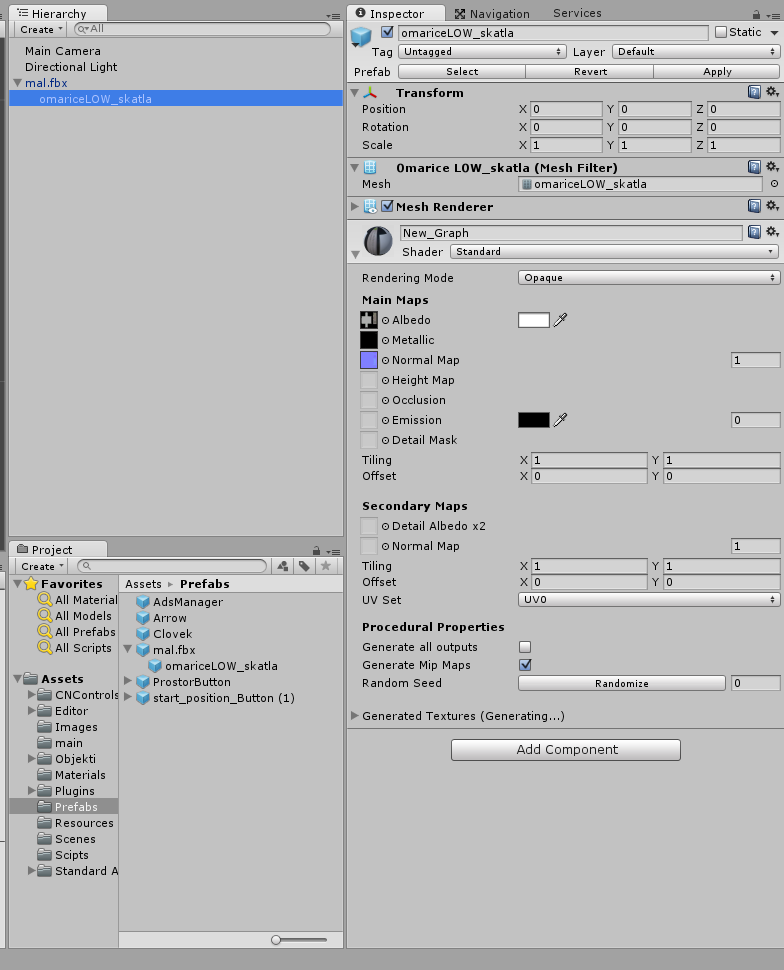
\includegraphics[width=9cm, height=12cm,keepaspectratio=true]{UnityPrefab2.png}
	\caption{Prefab spremembe}
\end{figure}
Prefabe se da zelo enostavno instancirati med igro. Kot spodaj vidimo. Narejenim objektom lahko tudi spreminjamo njihove lastnosti med igro.
\csharpsource{Izvorna_koda/Prefab.cs}